\documentclass[12pt]{article}
\usepackage{newcent} 
\usepackage[margin=3.3cm]{geometry}
\usepackage[utf8]{inputenc}
\usepackage[vietnamese]{babel}
\usepackage[tikz]{ocgx2}
\usepackage{xcolor}
\usepackage{pgfplotstable}
\usepackage{amsmath,amssymb,amsfonts}
\usepackage{graphicx}
\usepackage{pgfplots}
\usepackage{tikz}
\usepackage{subcaption}
\usepackage{changepage}
\usepackage{float}
\usepackage{hyperref}
\usepackage{pgfplotstable}
\usepackage{pgfplots}
\usepackage{blindtext}
\usepackage{titlesec}
\usepackage{array}
\usepackage{mathtools}
\usepackage{tabularx}
\usepackage{geometry}
\usepackage{nccmath}
\pgfplotsset{width=10cm, height=7cm}
\newtheorem{theorem}{Theorem}[section]
\newtheorem{corollary}{Corollary}[theorem]
\newtheorem{lemma}[theorem]{Lemma}
\setlength\tabcolsep{10pt}
\setlength\arraycolsep{10pt}
\setlength\extrarowheight{10pt}
\renewcommand{\labelenumii}{\arabic{enumi}.\arabic{enumii}}
\renewcommand{\labelenumiii}{\arabic{enumi}.\arabic{enumii}.\arabic{enumiii}}
\renewcommand{\labelenumiv}{\arabic{enumi}.\arabic{enumii}.\arabic{enumiii}.\arabic{enumiv}}
\newtheorem{dl}{Định lý}
\newtheorem{md}{Mệnh đề}
\newtheorem{bd}{Bổ đề}
\newtheorem{hq}{Hệ quả}
\newtheorem{cy}{Chú ý}
\begin{document}
\setlength{\parindent}{10pt}
%bia-start
\begin{titlepage}

    \begin{center}
    
    \textbf{\Large Trường Đại học Sài Gòn}
    
    \textbf{\Large Khoa Toán - Ứng dụng}
        
    \end{center}
    
    \vspace{2cm}
    
    \begin{center}
    
    \textbf{\huge BÀI TIỂU LUẬN GIỮA KÌ 1}
    
    \end{center}
    
    \vspace{1cm}
    
    \begin{center}
    
    \textbf{\huge ĐỀ TÀI (NHÓM 3)}

    \vspace{.5cm}
    
    \textbf{\huge [Tên đề tài]}
    
    \end{center}
    
    \vspace{1cm}
    
    \begin{center}
    
    \textbf{\Large Sinh viên thực hiện}
    
    \vspace{.5cm}

    \text{\Large Nguyễn Chí Bằng}
    
    \vspace{.4cm}

    \text{\Large 3122480004}
    
    \end{center}
    
    \vspace{1cm}
    
    \begin{center}
    
    \textbf{\Large Giảng viên hướng dẫn}
    
    \vspace{.5cm}

    \text{\Large TS. Nguyễn Văn Huấn}
    
    \end{center}
    
    \vspace{1cm}
    
    \begin{center}
    
    \text{\large Thành phố Hồ Chí Minh, năm 2023}
    
    \end{center}
    
    \end{titlepage}
%bia-end    
\title{ỨNG DỤNG VÀ CÁCH TẠO \\ THANG ĐO LIKERT}
\author{Nguyễn Chí Bằng}
\maketitle
\begin{abstract}
Trong phần này chúng ta sẽ tìm hiểu về ứng dụng của thang đo Likert đồng thời hướng dẫn chi tiết cách thức giúp người đọc có thể tạo và xử lý các vấn đề trong việc thu thập dữ liệu có sử dụng thang đo Likert. 
\end{abstract}

\tableofcontents

\section{Ứng dụng và ví dụ của thang đo Likert}
\phantom{}

Trong phần này, chúng ta sẽ khám phá ứng dụng của thang đo Likert trong nhiều lĩnh vực khác nhau, từ nghiên cứu khoa học đến quản lý tổ chức và thậm chí là trong việc đo độ hài lòng của khách hàng. Hãy cùng nhau tìm hiểu cách mà thang đo Likert không chỉ là một công cụ đo lường mà còn là một cầu nối quan trọng giữa nhà nghiên cứu và ý kiến của cộng đồng.

Có rất nhiều lĩnh vực có thể sử dụng thang đo Likert, tuy nhiên ta sẽ chỉ xem xét một số ví dụ có liên quan đến các lĩnh vực sau:
\begin{itemize}
    \item Khoa học thần kinh
    \item Dịch vụ
\end{itemize}

Mỗi ví dụ đều cho chúng ta thấy rằng thang đo Likert không chỉ là một công cụ đơn giản mà còn là một phương tiện đa dạng và hiệu quả trong việc thu thập thông tin ý kiến và đánh giá từ cộng đồng.

\subsection{Thang đo Likert trong khoa học thần kinh}
\phantom{}

Kết nối thông qua điện thoại thông minh và mạng xã hội giờ đây đã trở thành một phần không thể thiếu của nhiều người. Phần lớn mọi người đều có những trải nghiệm tích cực khi sử dụng mạng xã hội, nhưng nếu sử dụng quá mức sẽ gây ra những tác động tiêu cực đối với sức khỏe tâm thần lên người dùng. Nghiên cứu về lĩnh vực này vẫn đang ở những giai đoạn đầu, nhưng những nghiên cứu đều cho thấy tác động không nhỏ của mạng xã hội đến mọi người đặc biệt là giới trẻ.

Phương pháp sử dụng thang đo Likert giúp ta có cái nhìn trực quan cho vấn đề trên. Theo Risa Gelles-Watnick (một nhà phân tích nghiên cứu tập trung vào nghiên cứu internet và công nghệ tại Trung tâm Nghiên cứu Pew), khoảng ba phần tư thanh thiếu niên $(77\%)$ nói rằng họ sử dụng YouTube hàng ngày, trong khi một phần nhỏ hơn thanh thiếu niên $(58\%)$ nói điều tương tự về TikTok. Khoảng một nửa thanh thiếu niên sử dụng Instagram $(50\%)$ hoặc Snapchat $(51\%)$ ít nhất một lần một ngày, trong khi $19\%$ báo cáo sử dụng Facebook hàng ngày.

Một số thanh thiếu niên báo cáo sử dụng các nền tảng này gần như liên tục. Ví dụ, $19\%$ nói rằng họ sử dụng YouTube gần như liên tục, trong khi $16\%$ và $15\%$ nói tương tự về TikTok và Snapchat, tương ứng. (Hình \ref{mxh})

\begin{itemize}
\item Nguồn:
\begin{itemize}
\item Khảo sát được thực hiện từ ngày 14 tháng 4 đến ngày 4 tháng 5 năm 2022.
"Teens, Social Media and Technology 2022".
\item Thanh thiếu niên đề cập đến những người từ 13 đến 17 tuổi. Những người không đưa ra câu trả lời sẽ không được hiển thị.
\end{itemize}
\end{itemize}

\vspace{1cm}

\pgfplotstableread{
Place 1 2 3 4 5 6
\textbf{Facebook} 2 8 8 6 8 67
\textbf{TikTok} 16 32 9 5 4 33
\textbf{YouTube} 19 41 17 12 6 5
\textbf{Instagram} 10 27 12 7 5 38
\textbf{Snapchat} 15 29 7 3 5 41
}\testdata
\begin{figure}
\centering
\begin{tikzpicture}
    \begin{axis}[
                legend cell align=left,
                legend columns=3Z,
                legend style = {at={(0.5, -0.23)}, anchor=north, inner sep=3pt, style={column sep=0.15cm}},
                xbar stacked,
                xmin=0,
                xmax=100,
                xticklabel=\pgfmathprintnumber{\tick}\,$\%$,
                ytick=data,
                yticklabels from table={\testdata}{Place}
                ]
        %add descrip
        \addlegendimage{empty legend}
        \addlegendimage{empty legend}
        \addlegendimage{empty legend}
        \addlegendentry{}
        \addlegendentry{\textbf{Mức độ sử dụng}}
        \addlegendentry{}
        %add plot
        \addplot [fill=blue] table [x=1, meta=Place ,y expr=\coordindex] {\testdata};
        \addlegendentry{Liên tục}

        \addplot [fill=blue!70] table [x=2, meta=Place ,y expr=\coordindex] {\testdata};
        \addlegendentry{Thỉnh thoảng}

        \addplot [fill=blue!60] table [x=3, meta=Place ,y expr=\coordindex] {\testdata};
        \addlegendentry{1 lần/ngày}

        \addplot [fill=blue!50] table [x=4, meta=Place ,y expr=\coordindex] {\testdata};
        \addlegendentry{vài lần/tuần}

        \addplot [fill=blue!40] table [x=5, meta=Place ,y expr=\coordindex] {\testdata};
        \addlegendentry{Ít sử dụng}

        \addplot [fill=blue!30] table [x=6, meta=Place ,y expr=\coordindex] {\testdata};
        \addlegendentry{Không sử dụng}
    \end{axis}
\end{tikzpicture}
\caption{\centering $\%$ thanh thiếu niên Hoa Kỳ nói rằng họ truy cập hoặc sử dụng từng trang web hoặc ứng dụng trên.}
\label{mxh}
\end{figure}

\subsection{Thang đo Likert trong dịch vụ}
\phantom{}

Trong những năm gần đây khi khi sự cạnh tranh giữa các doanh nghiệp làm trong mảng dịch vụ ngày càng khốc liệt, việc đáp ứng và vượt qua mong đợi của khách hàng trở thành một trong những yếu tố quyết định sự thành công của mọi doanh nghiệp. Để đo lường và hiểu rõ hơn về mức độ hài lòng của khách hàng, các công ty và doanh nghiệp đã chọn sử dụng thang đo Likert trong quá trình đánh giá chất lượng dịch vụ do công ty cung cấp.

Việc sử dụng thang đo Likert trong dịch vụ, đặc biệt như đánh giá mức độ hài lòng của khách hàng giúp mang lại sự linh hoạt và chi tiết để đo lường ý kiến và cảm nhận. Thang đo Likert thường có một loạt các mức đánh giá từ tích cực đến tiêu cực, cho phép khách hàng chọn lựa mức độ đồng thuận hoặc phản đối của họ về một khía cạnh cụ thể của dịch vụ.

Amazon, một trong những đế chế thương mại điện tử lớn nhất thế giới, không chỉ nổi tiếng với việc cung cấp hàng hóa và dịch vụ đa dạng mà còn với sự tập trung mạnh mẽ vào khách hàng. Sau đây là mô hình khảo sát của Amazon có sử dụng thang đo Likert nhằm mục đích đưa ra quyết định về các vấn đề về quảng cáo hiển thị trên ứng dụng bằng cách khảo sát cảm nhận của người dùng. (Hình \ref{amazon})

$31\%$ người tiêu dùng nói rằng quảng cáo được tài trợ trong kết quả tìm kiếm là hữu ích. Chỉ có $20\%$ người tiêu dùng nói rằng những loại quảng cáo này gây mất tập trung.
\begin{itemize}
\item Nguồn:
\begin{itemize}
\item Dani Nadel (Chủ tịch và Giám đốc điều hành, Feedvisor).
\item Báo cáo Hành vi Người tiêu dùng Amazon năm 2021.
\end{itemize}
\end{itemize}
\pgfplotstableread{
Place 1
\text{Gây mất tập trung} 19.8
\text{Không tin tưởng} 4.0
\text{Không liên quan} 9.9
\text{Ít quan tâm} 17.5
\text{Không chắc} 6.4
\text{Phù hợp} 11.5
\text{Hữu ích} 30.9
}\testdata
\begin{figure}
\centering
\begin{tikzpicture}
    \begin{axis}[
                legend cell align=left,
                legend columns=3Z,
                legend style = {at={(0.5, -0.23)}, anchor=north, inner sep=3pt, style={column sep=0.15cm}},
                xbar stacked,
                xmin=0,
                xmax=35,
                xticklabel=\pgfmathprintnumber{\tick}\,$\%$,
                ytick=data,
                yticklabels from table={\testdata}{Place}
                ]
        %add plot
        \addplot [fill=green!50] table [x=1, meta=Place ,y expr=\coordindex] {\testdata};
    \end{axis}
\end{tikzpicture}
\caption{\centering $\%$ người tiêu dùng cảm thấy quảng cáo được tài trợ hữu ích trên ứng dụng mua hàng Amazon.}
\label{amazon}
\end{figure}

\section{Cách tạo thang đo Likert}
\phantom{}

Google form là công cụ tạo biểu mẫu giúp khảo sát thông tin bằng các câu hỏi trắc nghiệm hay tự luận. Mọi thông tin thu thập được từ Google form đều được sao lưu tự động giúp người dùng thực hiện một cách dễ dàng. Vì thế, việc sử dụng Google form để tiến hành tạo khảo sát bằng thang đo Likert là một lựa chọn tối ưu cho tất cả mọi người.

\vspace{1cm}

\subsection{Truy cập Google Form}

\vspace{.5cm}

Bước đầu tiên trong cách làm thang đo likert trong google form hiệu quả, bạn cần truy cập vào địa chỉ https://docs.google.com/forms/. Nếu chưa đăng nhập thì bạn cần phải đăng nhập, sử dụng tài khoản gmail để đăng nhập vào.

\begin{itemize}
\item Đến giao diện Google Form và click vào biểu tượng cửa sổ ở góc cùng bên phải và nhấn chọn Drive. 
\item Hệ thống sẽ tự động chuyển đến giao diện chính tại Google Drive. Tại đây, người thực hiện cần nhấn nút “Tạo mới” màu đỏ ở phía trái màn hình.
\end{itemize}

Sau khi đăng nhập, màn hình sẽ được hiển thị như hình \ref{1}
\begin{figure} 
    \centering
    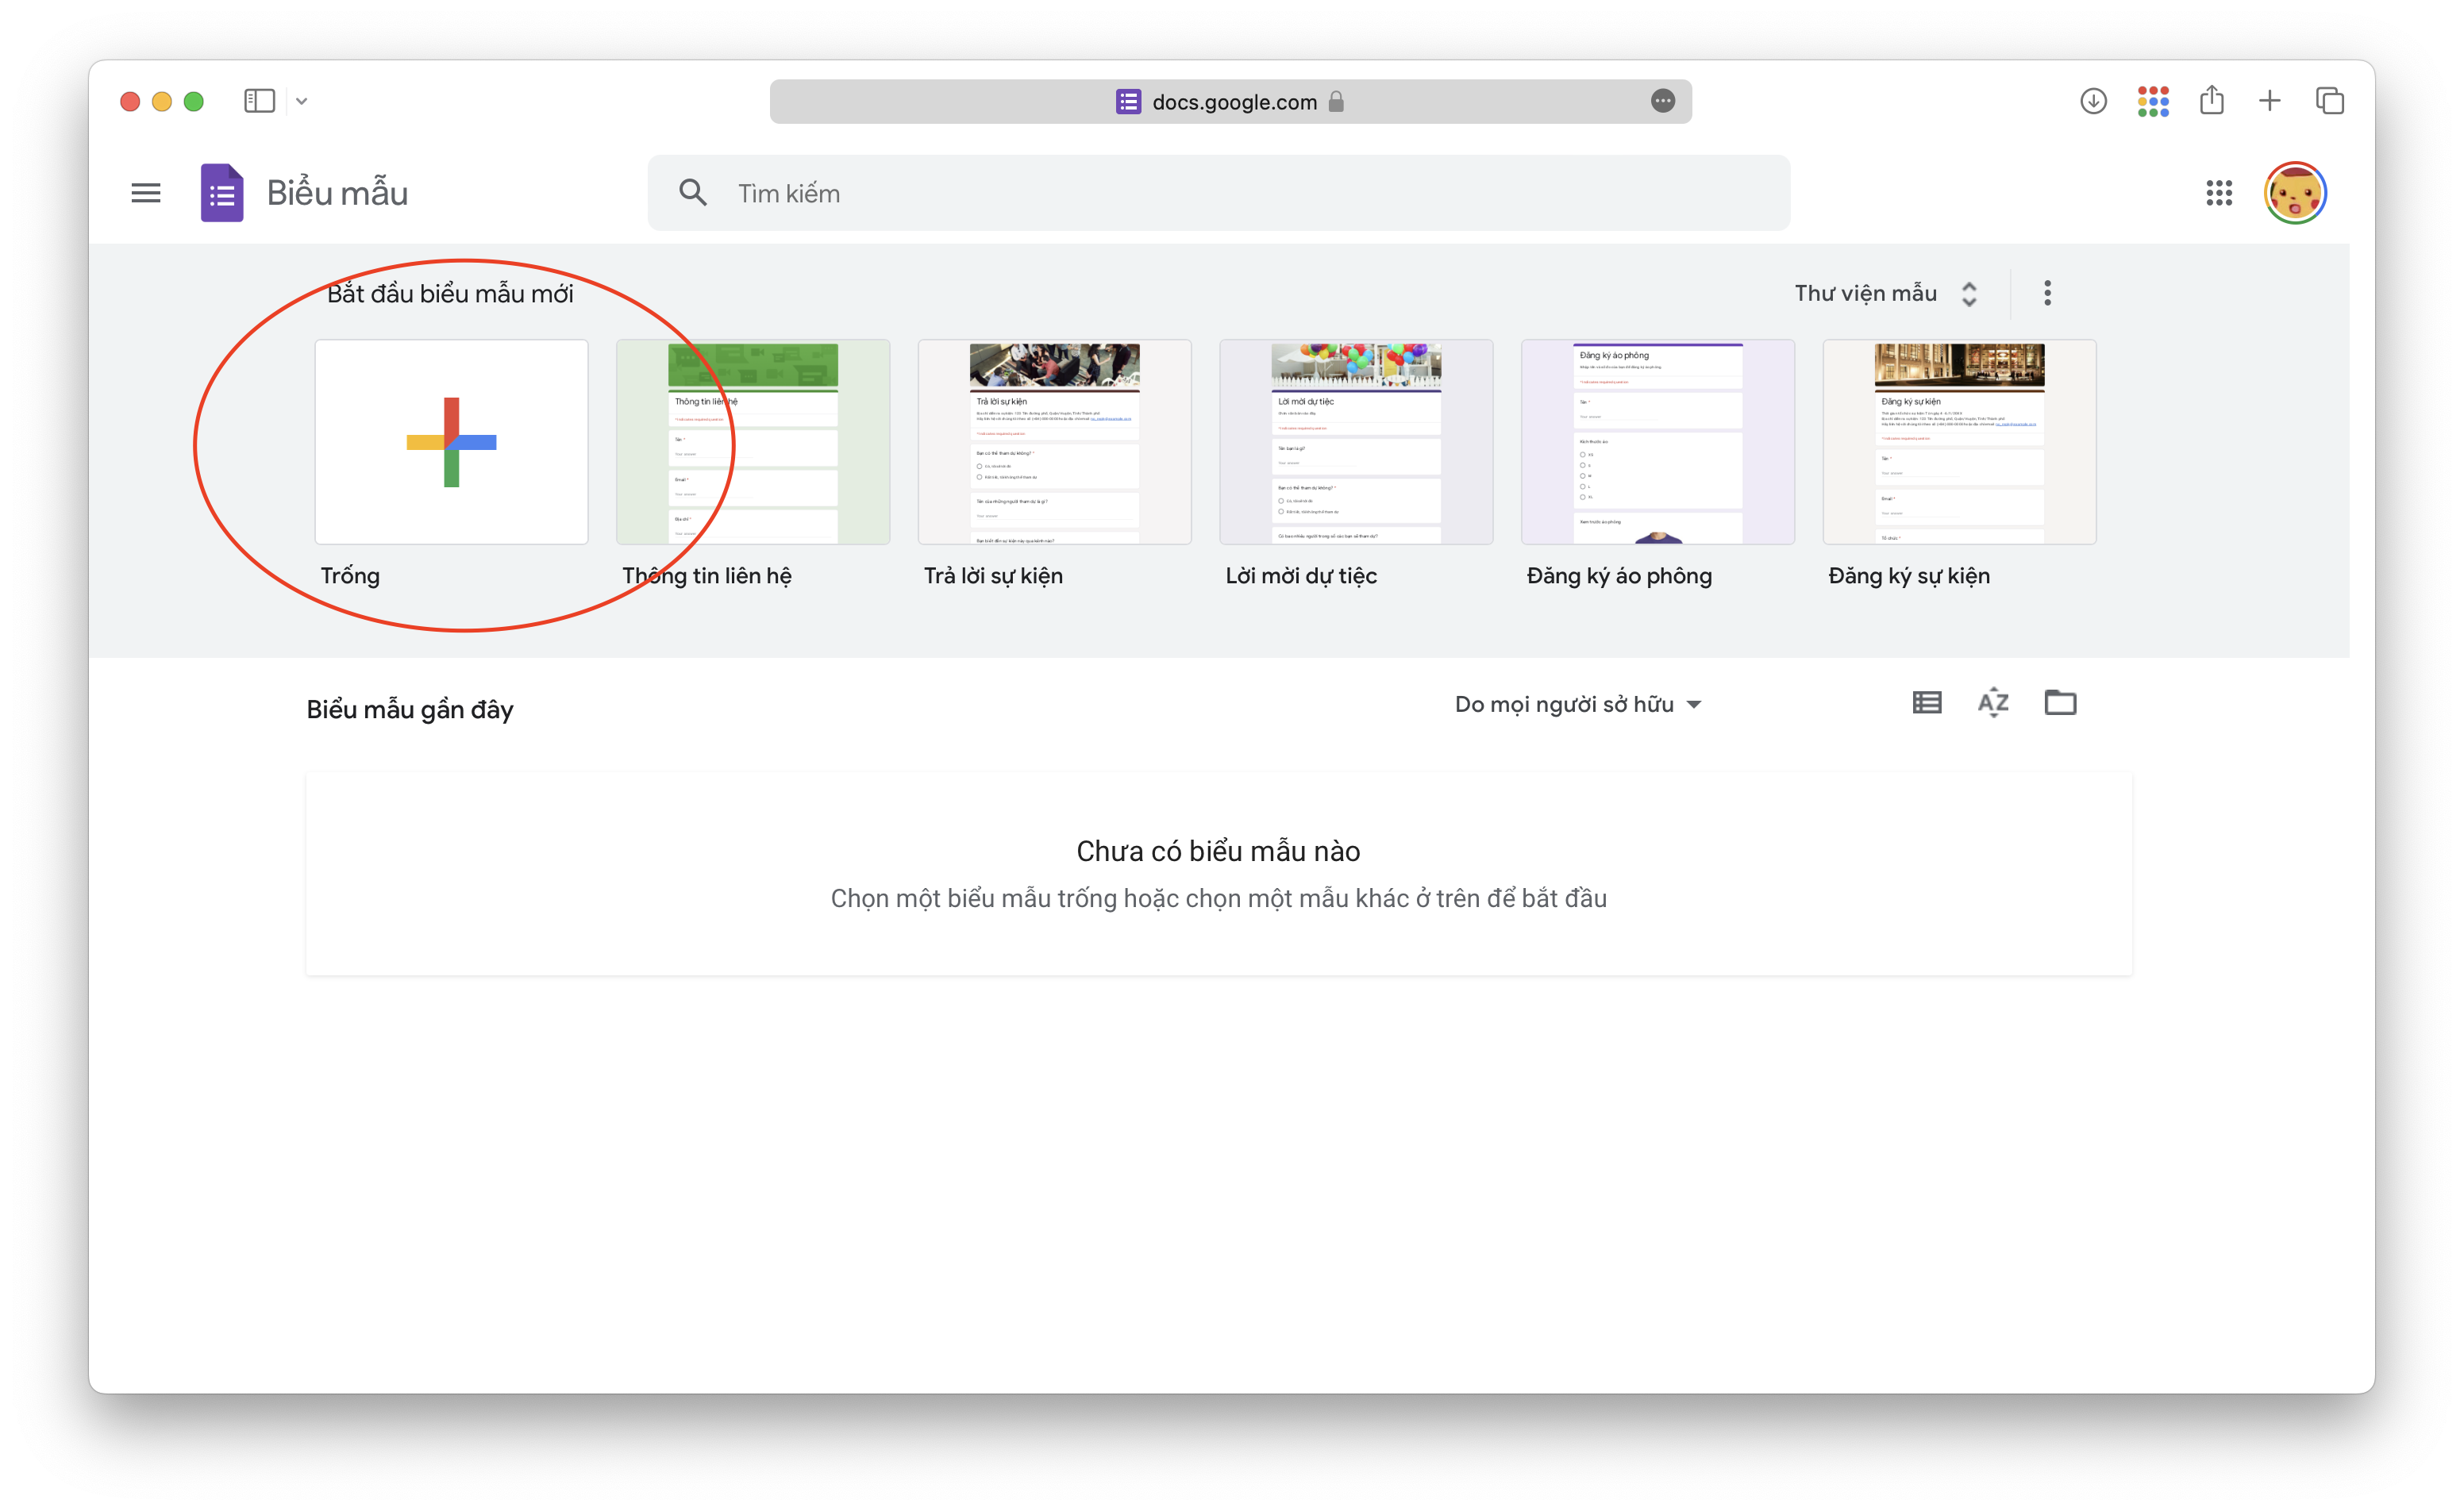
\includegraphics[width=0.7\linewidth]{/Users/chibangnguyen/Documents/GitHub/NCKH/thongkeud/tieuluan/Screenshot 2023-11-10 at 04.47.24.png}
    \caption{Giao diện chính tại docs.google.}
    \label{1}
\end{figure}

\vspace{1cm}

\subsection{Tạo form và điền thông tin}

\vspace{.5cm}

\begin{figure}
    \centering
    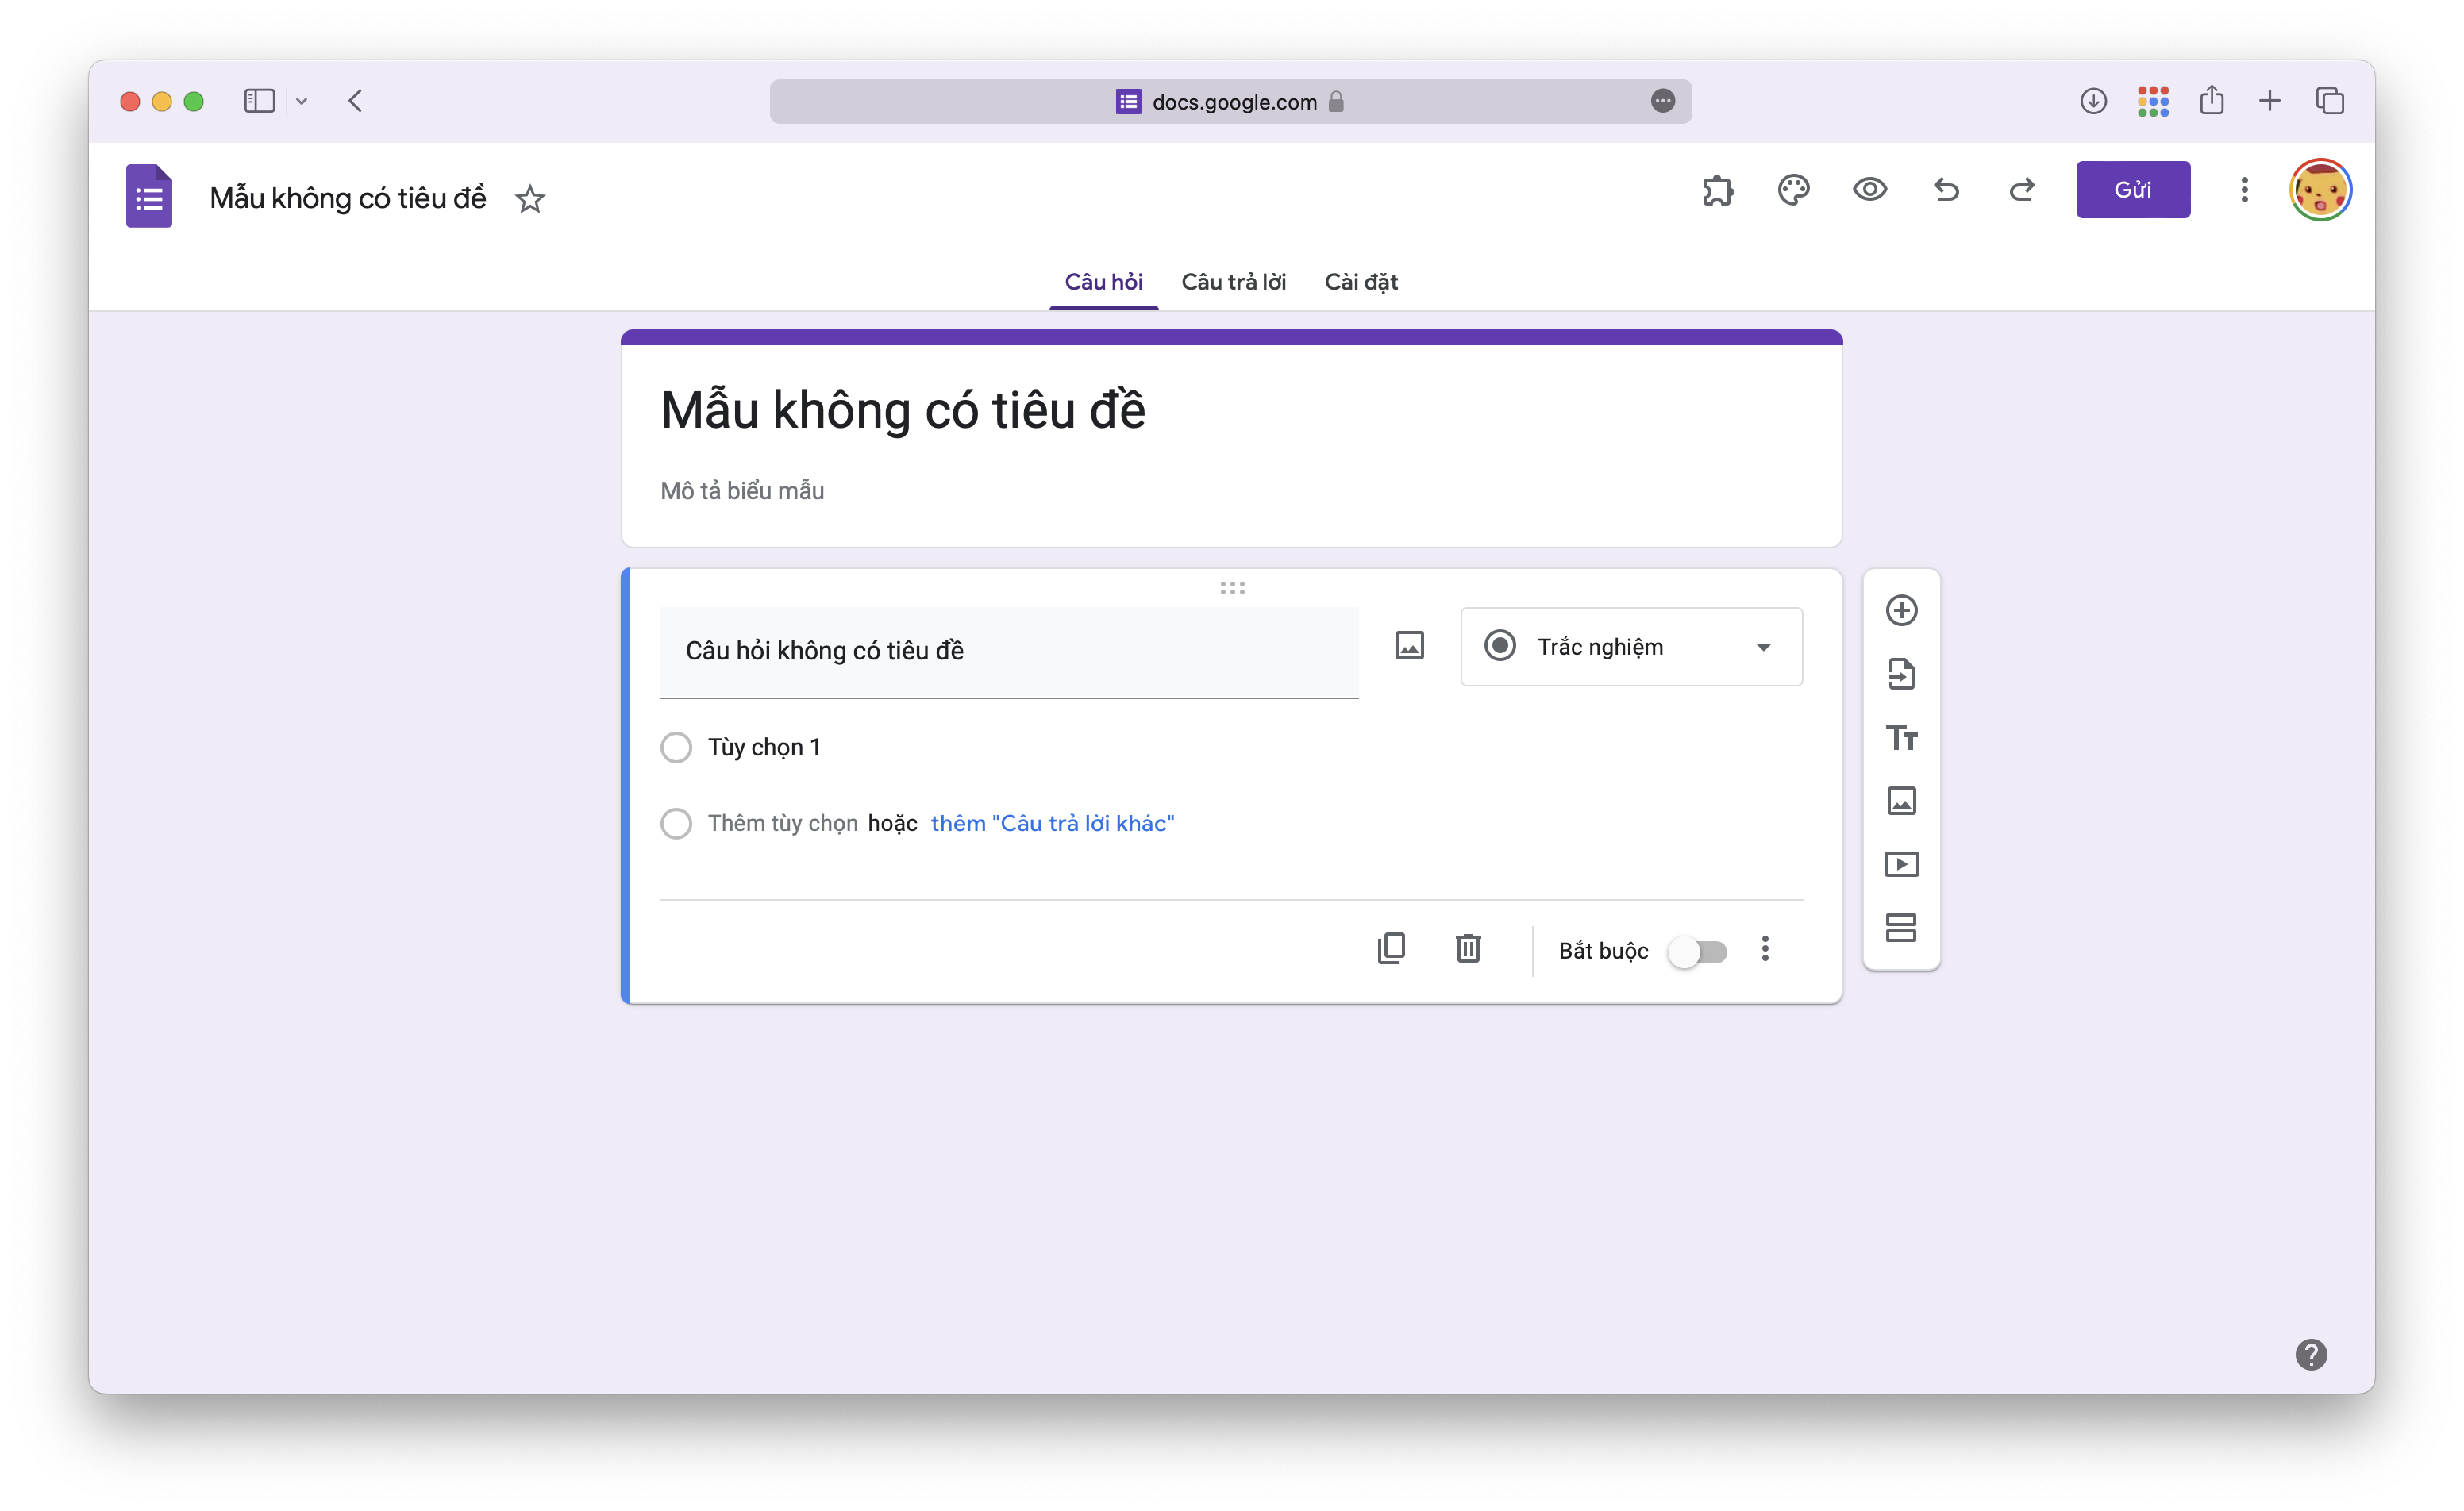
\includegraphics[width=0.7\linewidth]{/Users/chibangnguyen/Documents/GitHub/NCKH/thongkeud/tieuluan/Screenshot 2023-11-10 at 04.48.03.png}
    \caption{Form điền tiêu đề, tên và dạng câu hỏi trong cách làm thang đo likert trong google form.}
    \label{2}
\end{figure}

Form sẽ có dạng như sau (Hình \ref{2}), đây được coi là bước quan trong trong cách làm thang đo likert trong google form. Việc bạn cần làm là tạo tiêu đề form, tên câu hỏi và dạng câu hỏi. 

Trong cửa sổ mới, bạn nhập tiêu đề form để hoàn tất bước đầu tiên. Một lưu ý nhỏ, bạn cần chú ý tạo Title thu hút, hấp, chuyên nghiệp. Bạn cũng đừng quên điền phần mô tả để biểu mẫu được hoàn chỉnh nhất. 

Tạo câu hỏi: Đây là phần mọi người thắc mắc nhiều nhất trong cách làm thang đo likert trong google form. Các bước thực hiện sẽ được hiển thị ngay sau đây:

\begin{itemize}
\item Bạn hãy nhấp vào biểu tượng $(+)$ nằm tại vị trí đầu tiên trên thanh công cụ. 
\item Trên giao diện Google Form sẽ xuất hiện câu hỏi mới. Bạn tiến hành nhập nội dung câu hỏi và tùy chọn câu trả lời với kiểu tương ứng được xuất hiện trên giao diện.
\end{itemize}

Dưới đây bài viết sẽ hiển thị các dải lệnh câu hỏi được sử dụng phổ biến (Hình \ref{3}):

\begin{itemize}
\item Câu trả lời ngắn 
\item Câu trả lời bằng đoạn văn bản
\item Trả lời bằng câu đố, trắc nghiệm 
\item Hộp kiểm (Checkbox): Cho phép người được khảo sát chọn 1 hoặc nhiều tùy chọn. 
\item Menu thả xuống: Cho phép người dùng chọn giá trị từ danh sách đã có từ trước. 
\item Câu trả lời có phạm vi tuyến tính: Sử dụng cho các hỏi giúp đánh giá mức độ trong thang đo likert. 
\item Ngày và giờ trả lời.
\end{itemize}

\begin{figure}
    \centering
    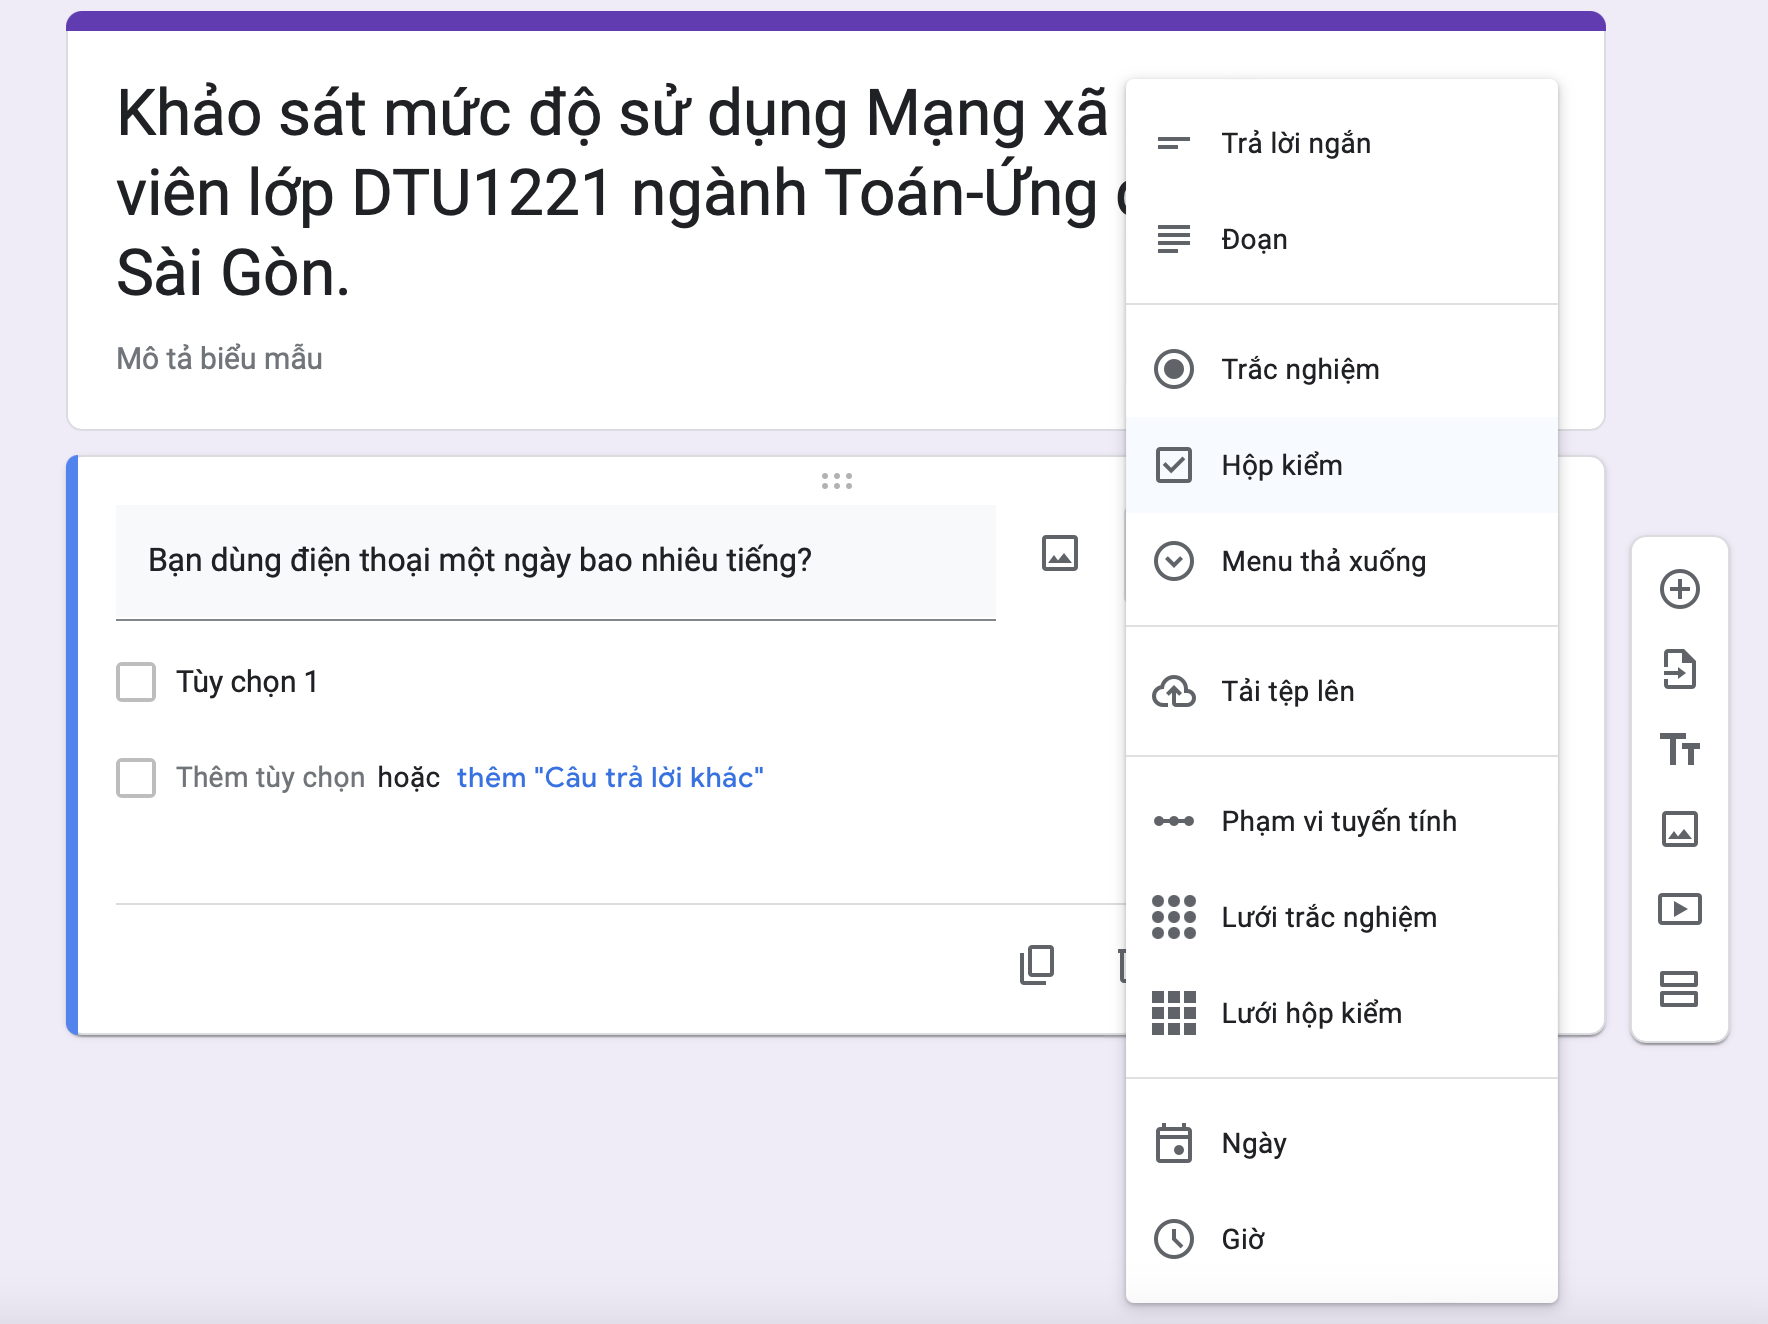
\includegraphics[width=0.7\linewidth]{/Users/chibangnguyen/Documents/GitHub/NCKH/thongkeud/tieuluan/Screenshot 2023-11-10 at 04.51.42.png}
    \caption{Hộp dải lệnh đầy đủ xuất hiện.}
    \label{3}
\end{figure}

Nếu muốn thay đổi vị trí hiển thị, bạn chỉ cần có thao tác kéo câu hỏi và di chuyển đến vị trí mình mong muốn. Hơn nữa, trên thanh công cụ ở góc dưới phần tạo câu hỏi cũng sẽ cung cấp một số tính năng khác như: sao chép câu hỏi, xóa câu hỏi… giúp bạn chỉnh sửa dễ dàng trong cách làm thang đo likert trong google form. 

\vspace{1cm}

\subsection{Tích chọn dạng câu hỏi là phạm vi tuyến tính}

\vspace{.5cm}

Các dạng câu hỏi sẽ tùy thuộc vào mục đích, đối tượng mà bạn muốn hướng đến khi thực hiện khảo sát để cho ra kết quả thấp nhất. Tuy nhiên trong cách làm thang đo likert trong google form, bạn nên chọn dạng câu hỏi là phạm vi tuyến tính. (Hình \ref{7})

\begin{figure}
    \centering
    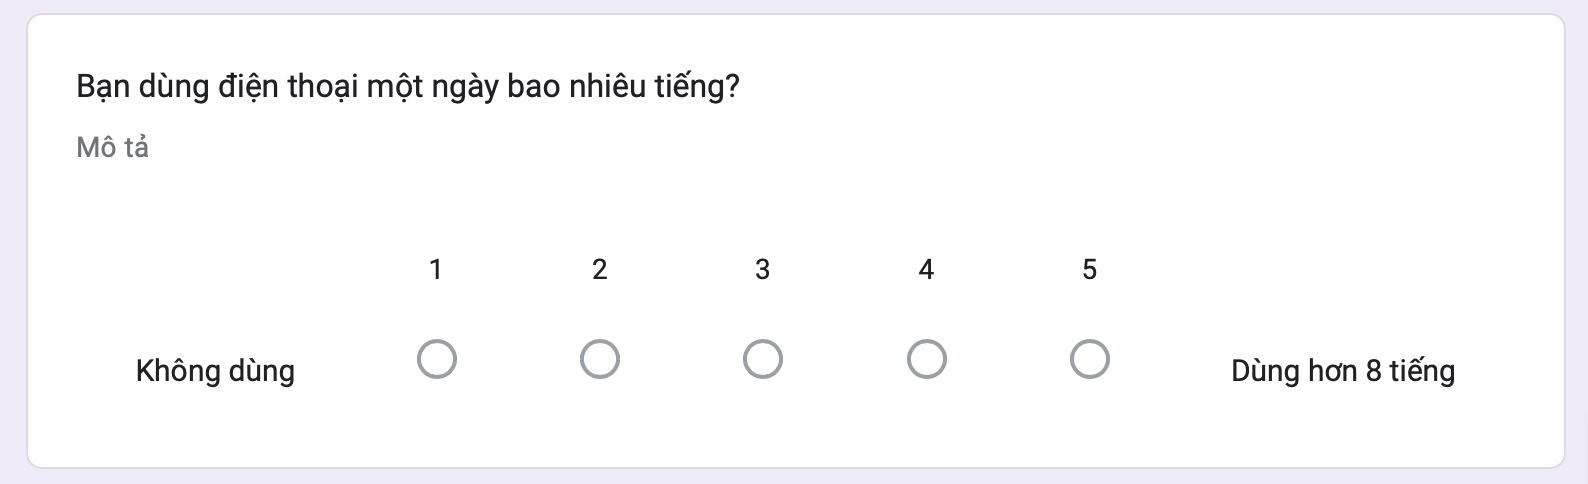
\includegraphics[width=0.7\linewidth]{/Users/chibangnguyen/Documents/GitHub/NCKH/thongkeud/tieuluan/Screenshot 2023-11-10 at 04.57.06.png}
    \caption{Lựa chọn Linear Scale để lập thang đo.}
    \label{7}
\end{figure}

\vspace{1cm}

\subsection{Chọn số mức thang đo (1-5, 1-7)}

\vspace{.5cm}

Đối với cách làm thang đo likert trong google form, chắc chắn bạn sẽ cần chọn số mức thang đo phụ thuộc vào số lượng câu hỏi mà bạn muốn khảo sát. Ngoài ra, để phân cách giữa các mục khác nhau, bạn cần click chuột vào biểu tượng tách biểu mẫu (nằm ở vị trí cuối cùng tại thanh công cụ bên phải màn hình). Ngay sau đó, các mục ở từng thang đo sẽ tách thành nhiều phần giúp người thực hiện khảo sát quan sát được dễ dàng, bạn cũng sẽ quản lý dữ liệu chính xác hơn. (Hình \ref{4})

\begin{figure}
    \centering
    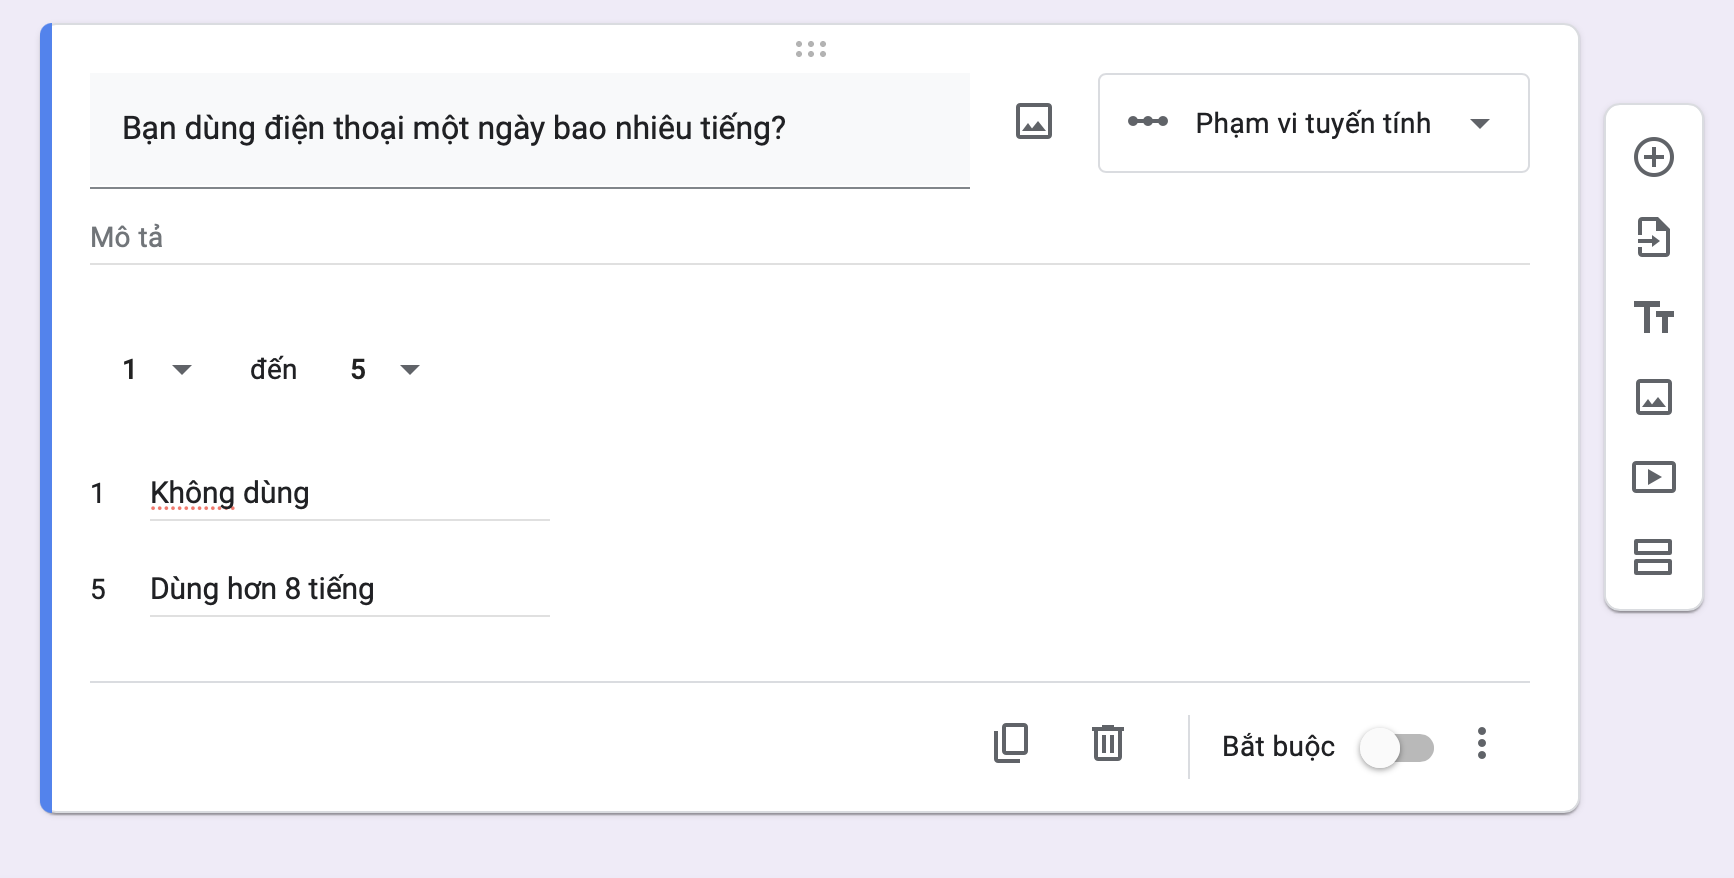
\includegraphics[width=0.7\linewidth]{/Users/chibangnguyen/Documents/GitHub/NCKH/thongkeud/tieuluan/Screenshot 2023-11-10 at 04.53.42.png}
    \caption{Chọn thang đo theo số phù hợp với mục đích.}
    \label{4}
\end{figure}

Nếu muốn bổ sung câu hỏi, bạn sẽ chỉ cần nhấn dấu cộng và làm lại bước 3 và chọn phạm vi tuyến tính và gõ lại biểu mẫu theo ý muốn. 

\vspace{1cm}

\subsection{Kiểm tra lại giao diện bảng câu hỏi}

\vspace{.5cm}

Sau khi thực hiện xong cách làm thang đo likert trong google form, bạn cần kiểm tra lần cuối và gửi cho đối tượng mà bạn muốn khảo sát. Khi họ mở ra, bạn hoàn toàn có thể theo dõi có bao nhiêu người, kết quả như thế nào vô cùng dễ dàng. Bạn sẽ vào mục CÂU TRẢ LỜI và nhấn chọn nút màu xanh như trong hình để tạo file excel hoặc google docs. (Hình \ref{5})

\begin{figure}
    \centering
    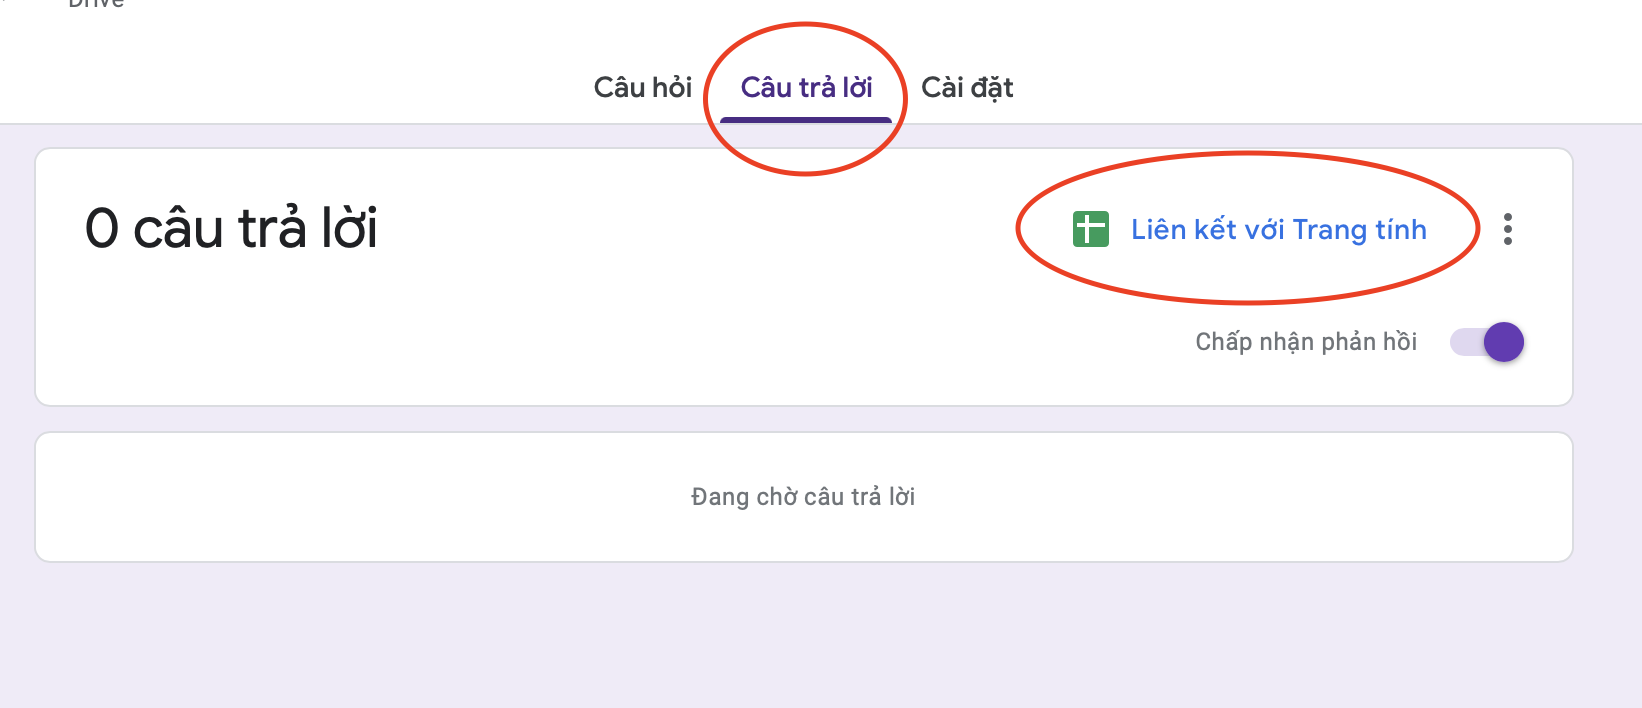
\includegraphics[width=0.7\linewidth]{/Users/chibangnguyen/Documents/GitHub/NCKH/thongkeud/tieuluan/Screenshot 2023-11-10 at 04.54.53.png}
    \caption{Kiểm tra lại giao diện bảng câu hỏi.}
    \label{5}
\end{figure}

Sau khi đã hoàn tất, công đoạn cuối khi gửi biểu mẫu đến những người tham gia bằng cách nhấn “Gửi” có màu tím ở góc bên phải màn hình. Có một giao diện mới sẽ hiển thị như sau: (Hình \ref{6})

\begin{figure}
    \centering
    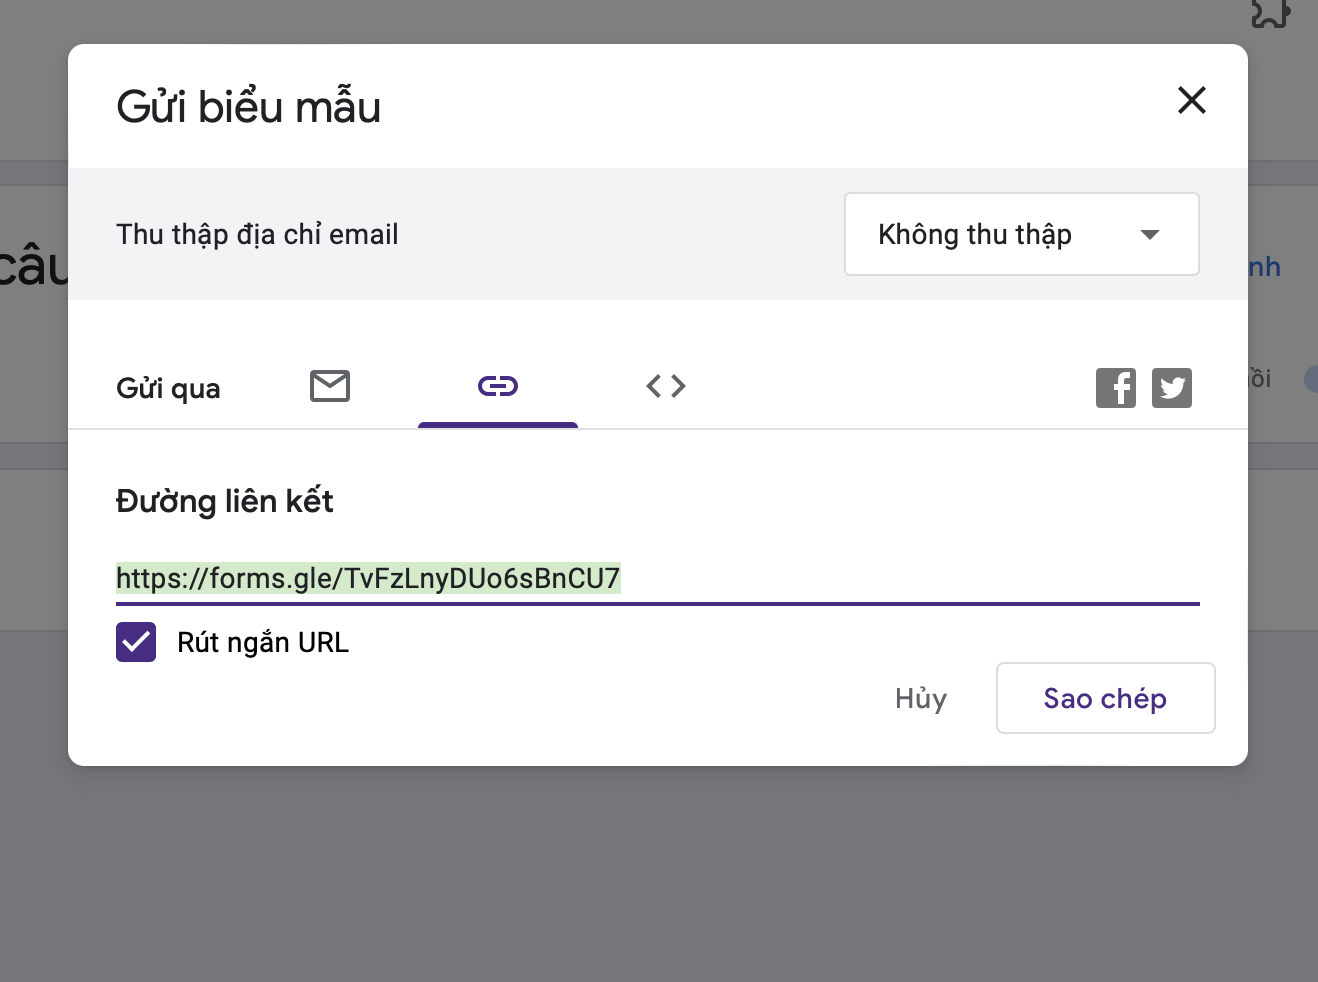
\includegraphics[width=0.7\linewidth]{/Users/chibangnguyen/Documents/GitHub/NCKH/thongkeud/tieuluan/Screenshot 2023-11-10 at 04.58.38.png}
    \caption{Copy link vừa tạo để gửi đi.}
    \label{6}
\end{figure}

\begin{itemize}
\item Gửi qua Email: Sẽ yêu cầu bạn có đầy đủ email, tiêu đề và lời nhắn đến với người nhận. 
\item Gửi qua URL: Bạn chỉ cần sao chép đường link và gửi đến người mà bạn muốn.
\item Gửi nhúng HTML: Bạn hoàn toàn thực hiện được trên các trang web hoặc Blog. 
\end{itemize}

Với các bước trong cách làm thang đo likert trong google form, bạn sẽ dễ dàng tiếp cận chính xác đối tượng cần khảo sát, kết quả cũng nhanh chóng trả về khi có người hoàn thành.

\end{document}